
\section{概観}

曲想, 調性, 構成その他多くの点でこの作品はベートーヴェンの第5番あるいは第9番と並べて論じられることが多い.
そこでまず最初にこれら3曲の比較を表\ref{comparison}にまとめておこう.

\begin{table}[htbp]
	\centering
	\begin{tabular}{c|cccc}
		& 第1楽章 & 第2楽章 & 第3楽章 & 第4楽章 \\ \hline
		LvB5 & ソナタ形式 & 変奏曲 & スケルツォ & ソナタ形式 \\
		& c-moll & As-Dur & c-moll & C-Dur \\ \hline
		LvB9 & ソナタ形式 & スケルツォ & 変奏曲 & -- \\
		& d-moll & d-moll & B-Dur & D-Dur \\ \hline
		JB1 & ソナタ形式 & 三部形式 & 三部形式 & ソナタ形式 \\
		& c-moll & E-Dur & As-Dur & C-Dur
	\end{tabular}
	\caption{LvB5, LvB9, JB1の比較}
	\label{comparison}
\end{table}

表\ref{comparison}から明らかなように, これら三曲はいずれも「暗から明へ」という基本的構造は共通であるが,
ブラームスとベートーヴェンとで中間楽章の調の選び方にはっきりとした相違がある:
ベートーヴェンは中間楽章のどちらか一方は主調である\footnote{ベートーヴェンの場合,
唯一第7番のみA-a-F-Aという調構造であり, 中間楽章に主調が現れない.}のに対して, ブラームスは (4曲すべての交響曲で) 中間楽章は主調と異なる調性を持つ.
また, ブラームスは中間楽章にベートーヴェン風のスケルツォを置いていない (第4番のみ第3楽章がスケルツォ風の音楽となっているが, それも2拍子である).

\begin{figure}[htbp]
	\centering
	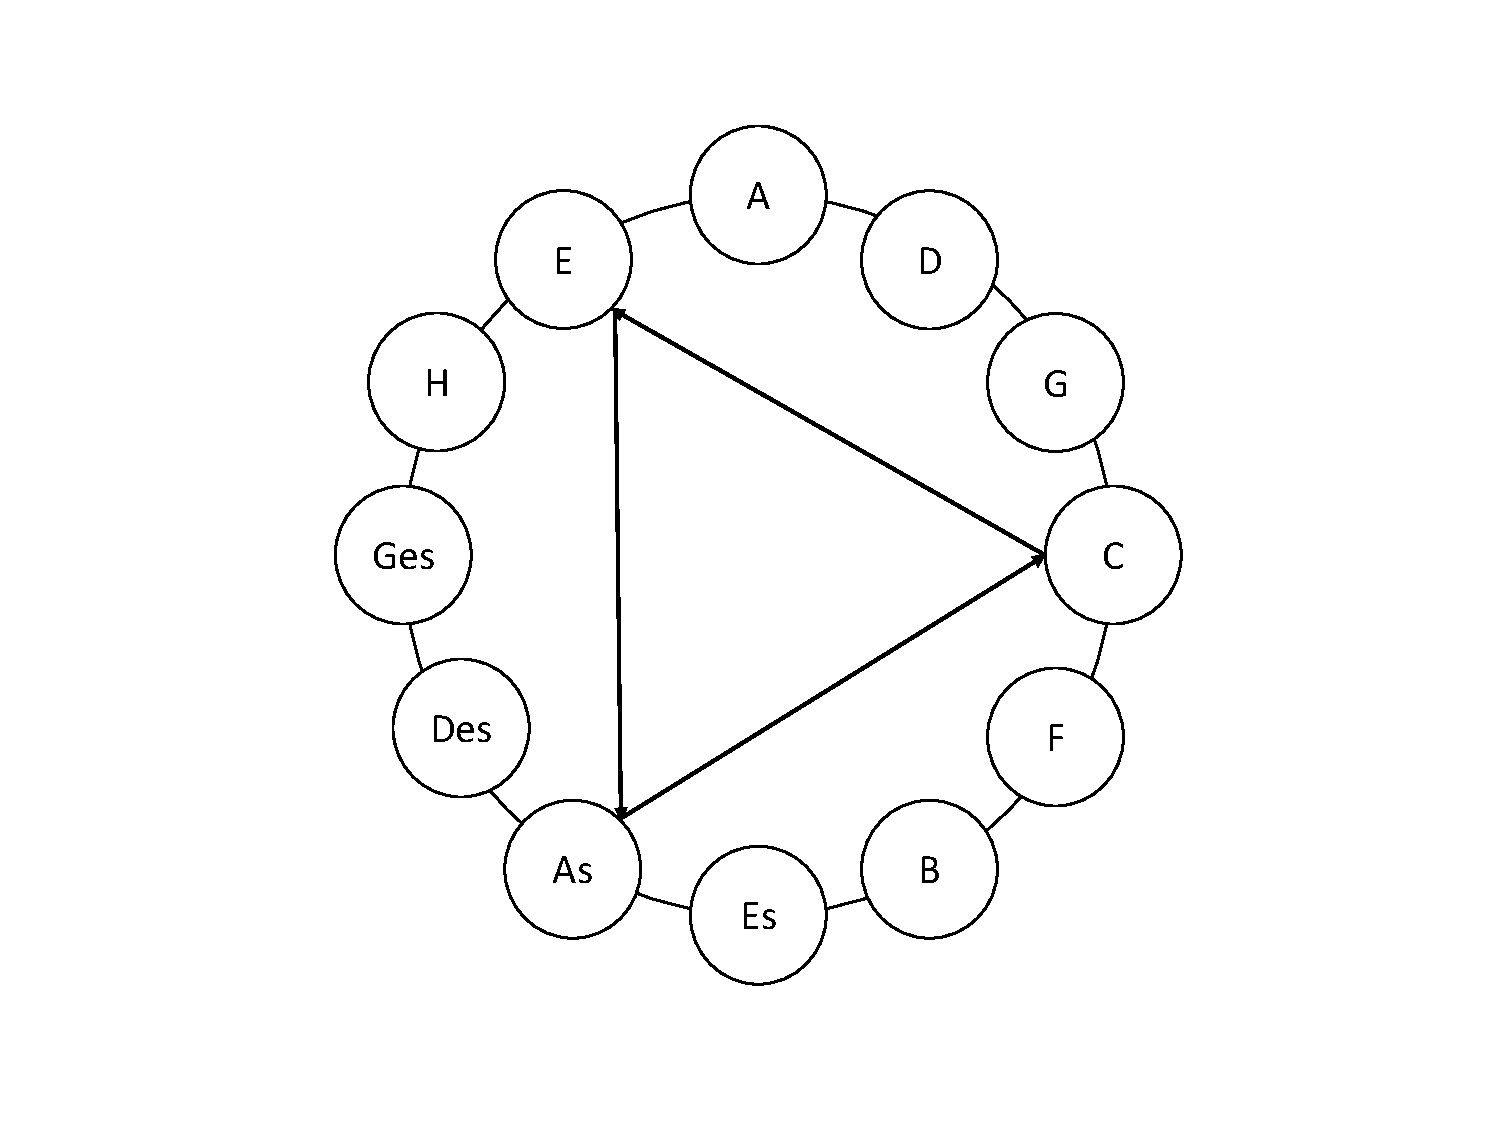
\includegraphics[clip,width=10.0cm]{./figure/modulatory.pdf}
	\caption{第1番の調構造}
	\label{modulatory}
\end{figure}

調性の観点からすると, ブラームスの第1番は彼の多くの作品の中でも独特の立ち位置を占めている:
C-E-As-Cという五度圏上の正三角形を描くような構成は他にない.
これらの調は互いに遠隔調の関係にあり, いずれも各楽章の最終和音の第3音を起点として自然に移行できる.

% 蛇足であるが, ブラームスの4つの交響曲の調性に関して次の事実がしばしば指摘される.
% これら4曲の調性はC-D-F-Eで, モーツァルトのジュピター音型に一致する. しかも, ロベルト・シューマンの4つの交響曲B-C-Es-Dを2度平行移動したものでもある.
% 筆者はこれについて単なる偶然の一致であり意味はないと解釈している:
% ブラームスのどの交響曲についても調性はその基本的性格から自然に決定されており, なんらかの意図で選ぶ余地はないように思われる.
% 特にシューマンの交響曲は単なる出版順であり作曲順は大きく異なっているし, ブラームスもそのことは十分承知していた.
